\chapter{Week}
All of the new information gathered at the Xilinx seminar last week needed to be transferred to the internal Wiki and properly documented. Three main tasks were worked upon in this week, namely preparing the second presentation 'Introduction to \ac{ML} on \ac{FPGA}', getting all of the \ac{DNNDK} sample applications to work on the ZCU 104 evaluation board and evaluating a possible collaboration with an ETH start-up called Synthara.
\begin{itemize}
	\item \textbf{Presentation:} Extensive market research has been conducted to find resources and ideas on how to present the different hardware platforms. The difficulty lies therein, that there are no standardized performance metrics for neural networks. Performance is strongly dependent on the network used and the individual use case. This leads to a lot of unfair comparisons, both in research and industry when numbers are shown. Therefore, a qualitative approach was chosen as doing all of these comparisons would have taken an extreme amount of work time and effort, requiring special hardware as well.
	\item \textbf{Bugfix for ZCU 104 evaluation board:} After reading through a vast amount of documentation and employing the help of online resources, mainly the Xilinx official forums, a solution was found to the problem. It turned out to be a specific problem of the ZCU 104 evaluation board which made it hard to track down. The solution to this was provided by an unofficial patch by on e of the Xilinx employees online. The board has power issues when running at full load resulting in the already mentioned problem of freezing the board in the middle of running the sample applications. After applying the patch all of the sample applications worked. These included image classification with resnet50 and inception-v1 as well as real time face detection, object detection and pose detection using other popular \ac{ANN}
	\item \textbf{Synthara collaboration:} During research for neural network accelerator implementations I read about an ETH start-up providing this service in the form of an \ac{ASIC}. However, their prototypes as a proof-of-concept are implemented on \acp{FPGA}. Thus, we reached out to them and scheduled a meeting. During this meeting we discussed the possibility of a cooperation. The idea was to implement a demonstrator for the Embedded World 2020 conference showing off Enclustra hardware and using the Synthara neural network accelerator. The demo is a game of rock-paper-scissors played by a human player against a robotic hand. The setup can be seen in figure~\ref{fig:demonstrator}. The robot hand is controlled via \ac{USB} using \ac{PWM} to control each finger individually. The human players movement is captured by a camera connected via \ac{MIPI} to the \ac{FPGA} board. The \ac{FPGA} handles all image preprocessing and is running a custom neural network capable of detecting hand gestures.
	\begin{figure}[!htb]
	\centering
		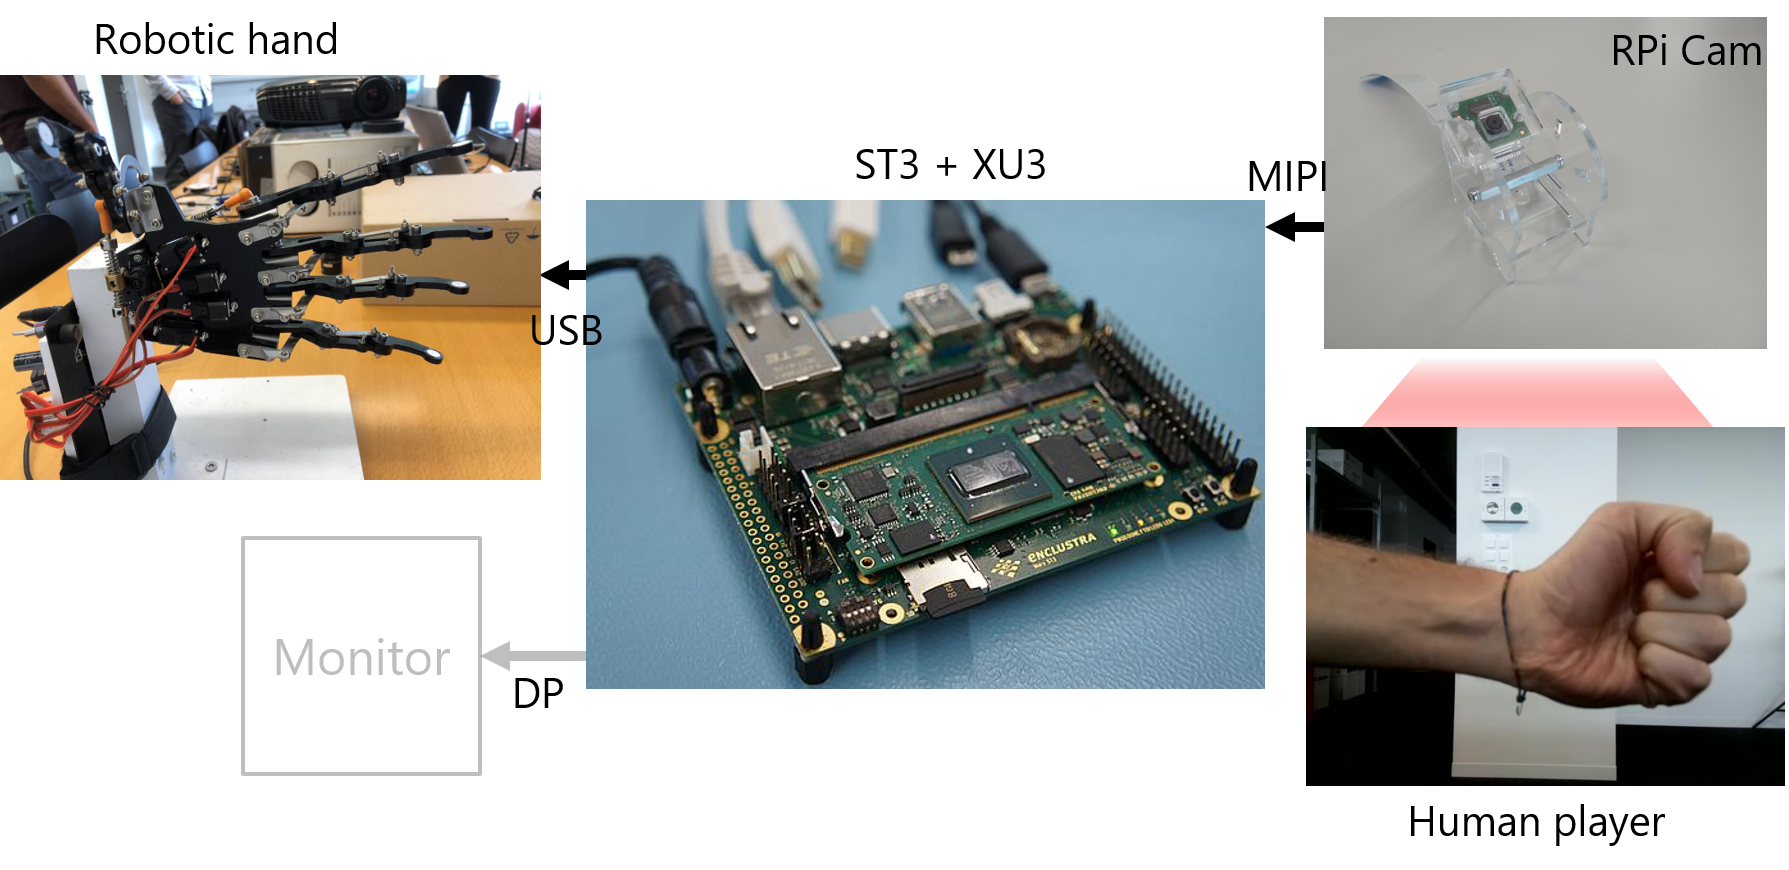
\includegraphics[width=\textwidth]{bilder/demonstrator.png}
		\caption{Rock-paper-scissors demonstrator setup}
		\label{fig:demonstrator}
	\end{figure}
\end{itemize}